
\section*{Security Controls, Mitigations, and Best Practices}
Effective threat modeling leads to actionable security controls. Security controls are technical, administrative, or physical safeguards designed to reduce risk by preventing, detecting, or responding to threats\cite{owasp,shostack2014}.

\subsection*{Authentication and Authorization}
	extbf{Definition:} Authentication verifies user identity; authorization determines access rights.\cite{owasp}
\begin{itemize}
	\item Multi-factor authentication (MFA)
	\item Strong password policies and storage (bcrypt, Argon2)
	\item Role-based access control (RBAC)
	\item Principle of least privilege
\end{itemize}

\subsection*{Input Validation and Output Encoding}
	extbf{Definition:} Input validation ensures only properly formed data enters the system; output encoding prevents injection attacks.\cite{owasp}
\begin{itemize}
	\item Validate all user input (whitelisting preferred)
	\item Use output encoding to prevent XSS
	\item Employ parameterized queries to prevent SQL injection
\end{itemize}

\subsection*{Data Protection}
	extbf{Definition:} Data protection involves safeguarding sensitive data at rest and in transit.\cite{nist800154}
\begin{itemize}
	\item Encrypt sensitive data in transit (TLS 1.3) and at rest (AES-256)
	\item Use secure cookies (HTTPOnly, Secure, SameSite)
	\item Mask sensitive data in logs
\end{itemize}

\subsection*{Monitoring and Incident Response}
	extbf{Definition:} Monitoring detects suspicious activity; incident response is the process of managing and mitigating security incidents.\cite{uceda2015}
\begin{itemize}
	\item Implement centralized logging and monitoring
	\item Set up alerting for suspicious activity
	\item Develop and test an incident response plan
\end{itemize}

\subsection*{Security Control Mapping Table}
\begin{table}[H]
\centering
\begin{tabular}{|l|l|l|}
\hline
	extbf{Threat} & \textbf{Control} & \textbf{Tool/Technique} \\
\hline
Spoofing & MFA, strong auth & Google Auth, Authy \\
Tampering & Input validation & OWASP ESAPI, ORM \\
Repudiation & Audit logs & ELK, Splunk \\
Info Disclosure & Encryption, access control & OpenSSL, GPG \\
DoS & Rate limiting, WAF & ModSecurity, Cloudflare \\
Privilege Escalation & RBAC, least privilege & IAM, sudoers \\
\hline
\end{tabular}
\caption{Mapping Security Controls to Threats\cite{owasp,shostack2014}}
\end{table}

\begin{figure}[H]
	\centering
	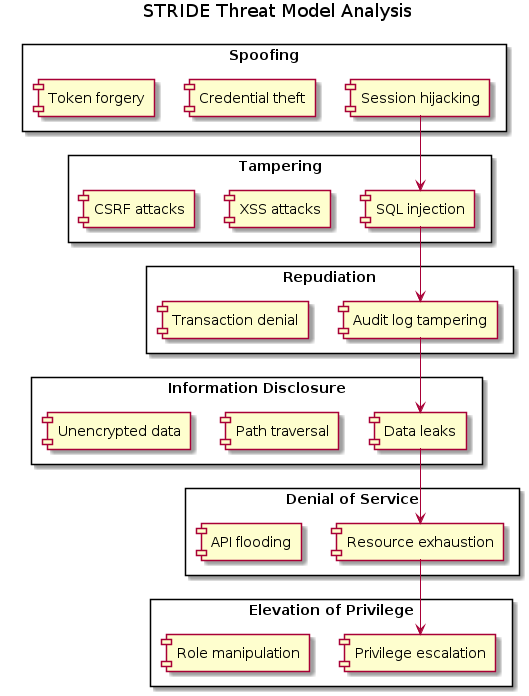
\includegraphics[width=0.7\textwidth]{images/stride-analysis}
	\caption{Security Controls Mapped to Threat Categories}
\end{figure}
